\nonstopmode
\documentclass[10pt,a4paper]{article}
\usepackage[utf8]{inputenc} % para poder usar tildes en archivos UTF-8
\usepackage[spanish]{babel} % para que comandos como \today den el resultado en castellano
\usepackage{a4wide} % márgenes un poco más anchos que lo usual
\usepackage{color}
\usepackage{gnuplottex}
\usepackage{amssymb}
%\usepackage{ccfonts,eulervm}
\usepackage{dot2texi}
\usepackage{tikz}
\usetikzlibrary{shapes,arrows}
\usepackage[T1]{fontenc}
\usepackage{listings}
\usepackage{xcolor}
\usepackage{amsmath}
\lstset { %
    language=C++,
    %backgroundcolor=\color{black!5}, % set backgroundcolor
                   basicstyle=\ttfamily,
                keywordstyle=\color{blue}\ttfamily,
                stringstyle=\color{red}\ttfamily,
                commentstyle=\color{green}\ttfamily,
                morecomment=[l][\color{magenta}]{\#}
}
\usepackage{float}
\usepackage{fancyhdr}
\pagestyle{fancy}
\thispagestyle{fancy}
\addtolength{\headheight}{1pt}
\lhead{AED3}
\rhead{RTP3}
\usepackage[ruled,vlined,linesnumbered]{algorithm2e}
\usepackage[conEntregas]{caratula}
\renewcommand*{\algorithmcfname}{Algoritmo}
\definecolor{dGray}{RGB}{100,100,100}

\begin{document}

\titulo{Reentrega del Trabajo Práctico III}
\subtitulo{Grupo 5}

\fecha{\today}

\materia{Algoritmos y Estructuras de Datos III}

\integrante{Aleman, Damian Eliel}{377/10}{damianealeman@gmail.com}
\integrante{Amil, Diego Alejandro}{68/09}{amildie@gmail.com}
\integrante{Barabas, Ariel}{775/11}{ariel.baras@gmail.com}
\integrante{Fern\'andez, Gonzalo Pablo}{836/10}{ralo4155@hotmail.com}

\maketitle


\tableofcontents

\newpage
\section{Algoritmo Exacto}
\subsection{Implementación del Algoritmo}

\par{Para realizar el algoritmo exacto, utilizamos la técnica de programación de
backtracking. Para ver cuál es el clique con una frontera de mayor
cardinalidad, calculamos la frontera de cada clique que hay en el grafo.
Partimos de una solución en la que el conjunto de nodos es vacío\footnote{
Es debatible si esta solución es válida o no, pero al tener frontera igual
a cero, cualquier solución válida con al menos uno de frontera será mejor.
En todo caso, si el grafo no tiene aristas, se devolverá esta solución vacía.}.
Luego utlizamos recursión para agregar cada posible nodo al conjunto. La
función recursiva se llama a sí misma dos veces: una agregando el i-ésimo
nodo a la solución actual y otra sin agregarlo.}\\

\par{A la función recursiva se le pasan como parámetros la solución actual y
la solución óptima hallada hasta el momento (ambas inicializadas con la
solución vacía). Cada vez que se entra a la función recursiva se evalúa el
tamaño de la frontera de la solución actual y si es mayor a la frontera de
la solución óptima, la solución actual reemplaza a la óptima. Una vez
finalizado el algoritmo se retorna la solución almacenada como óptima. La
solución vacía almacenada como óptima será reemplazada en cuanto se evalúe
cualquier solución con tamaño de frontera mayor a cero. Como cada nodo es una
clique, si el algoritmo retorna la solución vacía significa que el grafo no
tiene aristas.}\\

\par{Con el objetivo de reducir la complejidad del algoritmo exacto se ha
implementado una importante poda. Cuando la función va a llamarse
recursivamente, primero se evalúa si tiene sentido agregar el nodo a la
solución actual, es decir si con el nodo que se agrega, la solución actual
sigue representando una clique. Si con ese nodo no se
forma un clique, luego ese subconjunto de nodos sumado a otros nodos, tampoco
va a ser clique. Por esta razón, se poda toda solución que agregue el nodo
a la solución actual, es decir todo subconjunto de nodos, que no forman una
clique. A continuación se muestra un pseudocódigo del algoritmo exacto basado
en backtracking recursivo.}\\

\begin{algorithm}[H]
	\caption{Pseudocódigo del algoritmo exacto}
	\KwData{\textbf{Grafo} $G(V,E)$}
	\textbf{Solucion} $solucion\_optima$ $\leftarrow$ $solucion\_vacia$\\
	\textbf{Solucion} $solucion\_actual$ $\leftarrow$ $solucion\_vacia$\\
	Recursion(0, $solucion\_optima$, $solucion\_actual$)\\
	\textbf{return} $solucion\_optima$
\end{algorithm}

\begin{algorithm}[H]
	\caption{Llamada recursiva}
	\KwData{\textbf{int} $i$, \textbf{Solucion} $solucion\_optima$, \textbf{Solucion} $solucion\_actual$}
	$solucion\_optima$ $\leftarrow$ Max($solucion\_optima$, $solucion\_actual$)\\
	\If{$i$ = $cantNodos$}{
		Terminar recursion
	}

	\eIf{se\_conecta\_con\_clique($i$, $solucion\_actual$)}{
		Agregar $i$ a $solucion\_actual$\\
		Recursion($i+1$, $solucion\_optima$, $solucion\_actual$)\\
		Quitar $i$ de $solucion\_actual$\\
		Recursion($i+1$, $solucion\_optima$, $solucion\_actual$)
	}{
		Recursion($i+1$, $solucion\_optima$, $solucion\_actual$)
	}
\end{algorithm}

\par{La función $Max$ compara dos soluciones y retorna la de mayor frontera.
$cantNodos$ es la cantidad de nodos del grafo. Cuando el índice del nodo que se
va a agregar $i$ es igual a dicha cantidad, significa que ya no hay más nodos
para agregar y la recursión debe terminar. En otras palabras, se llegó a una
hoja del árbol de backtracking. La función $se\_conecta\_con\_clique$ toma un
nodo $i$ y una solución $S$ y retorna si la solución $S$ seguiría representando
una clique tras agregarle el nodo $i$. Para ello evalúa si existe una arista
entre el nodo $i$ y cada nodo de la clique representada por $S$.}

\subsection{Orden de complejidad}

\par{No puede hacerse mucho análisis respecto al orden de complejidad. El
algoritmo exacto recorre todas las posibles soluciones. Si bien hemos
implementado una poda, en el peor caso (un grafo completo $K_n$) todas las
soluciones serán válidas y todas ellas deberán ser evaluadas. Dado que en
una solución cada nodo puede estar o no estar, la cantidad de soluciones
posibles (la cantidad de subconjuntos del conjunto de nodos) es $2^n$ con
$n$ la cantidad de nodos. Las operaciones realizadas para cada solución son
polinomiales y, por lo tanto no aportan a la complejidad exponencial. La
función $se\_conecta\_con\_clique$ compara $k$ elementos con $k$ la cantidad
de nodos del conunto, que es a lo sumo $n$. Cuando se agregan o se quitan
nodos de una solución, la frontera de dicha solución debe recalcularse. La
complejidad de agragar o quitar un nodo $i$ es $d_G(i)$ (el grado de dicho
nodo, que también puede acotarse superiormente por $n$), ya que deben
evaluarse todas sus aristas. En definitiva, la complejidad del algoritmo
exacto es $2^n * ( n + n + n ) \in$ O($2^n$)}

\subsection{Experimentación}

\subsubsection{Performance}

\par{El archivo $test\_exacto.cpp$ en la carpeta $codigo/exacto$ contiene la
implementación del código que mide los tiempos de ejecución del algoritmo
exacto. Se ejecutó este programa con $N$ = 50,\\$s$ = 1 y $k$ = 10. Es decir,
para cada $n$ entero entre 1 y 50, se generaron 10 grafos aleatorios (
con la función $generar\_aristas\_aleatorias$). Para cada instancia generada se
corrieron dos verisones del algoritmo exacto. Uno con la poda y otro sin ella.
En el siguiente gráfico se muestran los resultados obtenidos.}

\begin{center}
\textbf{Gráfico de performance del algoritmo exacto en\\función de la cantidad
de nodos del grafo}
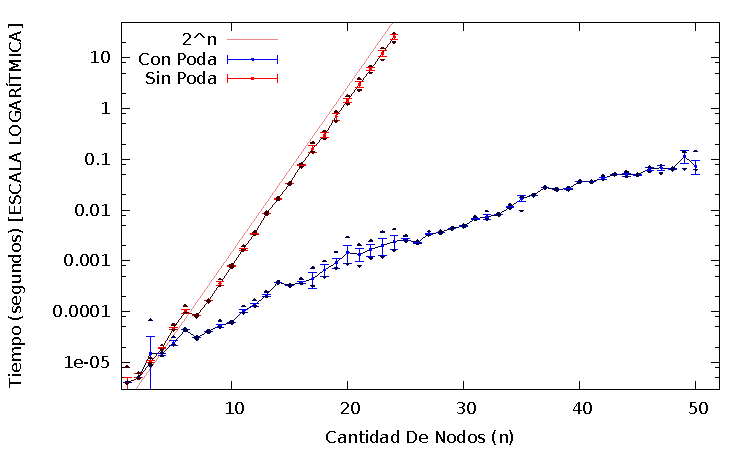
\includegraphics[scale=1.3]{imgs/exacto_50_1_10.pdf}
\end{center}

\par{Cada punto $\bullet$ en el gráfico representa el promedio de los tiempos
medidos para cada una de las 10 ejecuciones de una determinada cantidad de nodos
del grafo. El tamaño del segmento vertical sobre cada punto $\bullet$ representa
su varianza asociada. Además, para cada cantidad de nodos $n$ se graficaron la
máxima medición con $\blacktriangle$ y la mínima medición con
$\blacktriangledown$.}\\

\par{La función graficada con una curva sin puntos es una función exponencial de
base 2. Al estar utilizando escala logarítmica en el eje de ordenadas, esta curva
se ve como una recta. Como se puede observar, la curva definida por la versión
sin poda del algoritmo (la curva resultante de unir los puntos $\bullet$) se
asemeja mucho a tal curva. Mientras que la versión con poda tiene
menores tiempos promedio de ejecución, si bien tiene la misma complejidad.}\\

\par{En la mayotía de los casos, la varianza de ambas versiones es tan pequeña
que apenas puede verse en el gráfico. Esto nos dice que ambas versiones del
algoritmo son estables. Era de esperarse de la versión sin poda, ya que dado
cualquier grafo, la cantidad de soluciones que deben recorrerse es siempre
la misma. Sin embargo, de la versión con poda se esperaba una varianza bastante
superior debido a que la cantidad de soluciones que este debe recorrer depende
en gran medida del grafo entrada.}


\newpage
\section{Apéndice}

\subsection {La clase Grafo}
\begin{lstlisting}
struct arista{
	int nodo1;
	int nodo2;
	
	arista(int n, int m){
		this->nodo1 = n;
		this->nodo2 = m;
	}

};

class grafo
public:
 int cantNodos;
 vector< vector<int> > lista_global;
 vector< vector<int> > matriz_ady;
 vector<arista> aristas;

 //Constructor: Construye un grafo vacío
 grafo(){
  grafo(0);
 }

 //Constructor: Construye un grafo con n nodos sin aristas
 grafo(int n){
  constructor(n);
 }

 //Construye el grafo a partir de la entrada estandar
  // (llamar despues del constructor vacío)
 void inicializar() {
  int n, m, a, b, c;
  cin >> n;
  constructor(n);
  if(n != 0) {
   cin >> m;
   for(int i = 0; i < m; ++i){
    cin >> a;
    cin >> b;
    //Paso de 1..n a 0..n-1::
    a--; b--;
    asociar(a,b);
   }
  }
 }

 //Construye un grafo con aristas aleatorias
  // (llamar despues del constructor basico)
 void generar_aristas_aleatorias() {
  srand(time(NULL));
  for(int i = 0; i < cantNodos; ++i)
  for(int j = i; j < cantNodos; ++j)
   if(rand() \%2 == 0) asociar(i, j);
 }

 int gradoMax(){
  unsigned int gradoMax = 0;
  for (int i = 0; i < cantNodos; ++i ){
   if (lista_global[i].size() > gradoMax) {
    gradoMax = lista_global[i].size();
   }
  }
  return gradoMax;
 }

 int grado(int i) {
  return lista_global[i].size();
 }

 void asociar(int nodo1, int nodo2){

  if(nodo1 != nodo2){

   /* Agrego la arista faltante  */
   this->aristas.push_back(arista(nodo1,nodo2));
   
    //agrego cada nodo en la lista del otro nodo incidente
     
    (this->lista_global[nodo1]).push_back(nodo2);
    (this->lista_global[nodo2]).push_back(nodo1);
  
    (this->matriz_ady[nodo1][nodo2]) = 1;
    (this->matriz_ady[nodo2][nodo1]) = 1;
  }
 }
 
 bool hayArista(int nodo1, int nodo2) const{
  return (matriz_ady[nodo2][nodo1] == 1);
 }

 // Devuelve si el nodo 'nodo' se conecta con la clique 'clique'
 bool se_conecta_con_clique(int nodo, vector<bool> &clique){
  for (int i = 0; i < cantNodos; ++i) {
   if ( (clique[i]) && (matriz_ady[i][nodo]==0) ){
    return false;
   }
  }
  return true;
 }

 // Devuelve si el conjunto 'nodos' representa una clique
 bool es_clique(vector<bool> nodos) {
  vector<int> clique = vector<int>();
  for (int i=0; i<cantNodos; i++) {
   if (nodos[i]) {
    for (int j=0; j<clique.size(); j++) {
     if(matriz_ady[i][clique[j]]==0) return false;
    }
    clique.push_back(i);
   }
  }
  return true;
 }

 // Determina cuanto varía la frontera de la clique 'clique'
  // al agregar el nodo 'nodo'
 int cuanto_aporta(int nodo, Solucion &s){
  int frontera_inicial = s.second;
  alternar(s, nodo);
  int frontera_final = s.second;
  alternar(s, nodo);
  return frontera_final - frontera_inicial;
 }

 // Devuelve el v-esimo vecino de la solucion s
 Solucion obtener_vecino(Solucion &s, Solucion &vAnterior, int v) {
  Solucion vecino;
  int nodos_distintos = 1;//Me dice cuantos nodos debo agregar/sacar
  int vecinos = combinatorio(cantNodos,1);
  while (v >= vecinos) {
   nodos_distintos++;
   v -= vecinos;
   vecinos = combinatorio(cantNodos, nodos_distintos);
  }
  if (v==0) {
   vecino = make_pair(s.first, s.second);
   for (int i=0; i<nodos_distintos; i++) {
    alternar(vecino, i);
   }
  } else {
   vecino = make_pair(vAnterior.first, vAnterior.second);
   if (vecino.second < 0) vecino.second*=-1;
   int ov = 0;
   for (int i=cantNodos-1; i>=0; i--) {
    if (s.first[i]!=vAnterior.first[i]) {
     if (i==cantNodos-1-ov) {
      ov ++;
      alternar(vecino, i);
     } else {
      if (ov>0) {
       alternar(vecino, i);
       alternar(vecino, i+1);
       int j = i+2;
       while(ov>0 && j<cantNodos && vecino.first[j]==s.first[j]) {
        alternar(vecino, j);
        j++; ov--;
       }
       if (ov==0) break;								
      } else {
       alternar(vecino, i);
       alternar(vecino, i+1);
       break;
      }
     }
    }
   }
  }
  if (!es_clique(vecino.first)) vecino.second *= -1;
  return vecino;
 }

 void alternar(Solucion &v, int i) {
  v.first[i] = !v.first[i];
  //Recalcular vecino.second (frontera) en funcion del nodo
  // sacado/agregado (no importa si es o no una clique, todavía)
  if (v.first[i]) {
   for (int j=0; j<lista_global[i].size(); j++) {
    if (v.first[lista_global[i][j]]) {
     v.second--;
    } else v.second++;
   }
  } else {
   for (int j=0; j<lista_global[i].size(); j++) {
    if (v.first[lista_global[i][j]]) {
     v.second++;
    } else v.second--;
   }			
  }
 }
 
private:
 void constructor(int n) {
  //cargo la cantidad de nodos
  this->cantNodos = n;

  vector <int> vec;

  //inicializo todas las listas vacias
  for(int i = 0; i < n; i++){
   (this->lista_global).push_back(vector <int>()) ;
  }

  for(int i = 0; i < n; i++){
   (this->matriz_ady).push_back(vector <int>(n)) ;
  }
 }
\end{lstlisting}
\newpage
\subsection{Algoritmo Exacto}

\begin{lstlisting}
Solucion exacto(grafo &g) {
Solucion optima = make_pair(vector<bool>(g.cantNodos,false), 0);
Solucion actual = make_pair(vector<bool>(g.cantNodos,false), 0);
exacto_recur(g, 0, optima, actual);
return optima;
}

Solucion exacto_sin_poda(grafo &g) {
Solucion optima = make_pair(vector<bool>(g.cantNodos,false), 0);
Solucion actual = make_pair(vector<bool>(g.cantNodos,false), 0);
exacto_recur_sp(g, 0, optima, actual);
return optima;
}

void exacto_recur(grafo &g, int i, Solucion &optima, Solucion &actual) {
if (actual.second > optima.second) {
 optima = actual;
}
if (i==g.cantNodos) {
 return;
}

// si se conecta_con_clique sigo la recursion con y sin ese nodo
if ( g.se_conecta_con_clique(i, actual.first) ) {
 g.alternar(actual, i);
 exacto_recur(g, i+1, optima, actual);
 g.alternar(actual, i);
 exacto_recur(g, i+1, optima, actual);
// si no se conecta con mas nodos tampoco va a ser una clique,
// luego hago la recursion sin ese nodo
}else{
 exacto_recur(g, i+1, optima, actual);
}
}

void exacto_recur_sp(grafo &g, int i, Solucion &optima, Solucion &actual) {
if (actual.second > optima.second) {
 optima = actual;
}
if (i==g.cantNodos) {
 return;
}
g.alternar(actual, i);
exacto_recur_sp(g, i+1, optima, actual);
g.alternar(actual, i);
exacto_recur_sp(g, i+1, optima, actual);
}
\end{lstlisting}

\newpage
\subsection{Heur\'istica Golosa}
\begin{lstlisting}
Solucion goloso(grafo g){
Solucion s = make_pair(vector<bool>(g.cantNodos,false), 0);

while (true){
 int candidato = -1;
 int maximo_aporte = 0;

 // veo cual es el nodo que mas aporta y si aporta algo
  // positivo, lo agrego
 for (int i = 0 ; i < g.cantNodos; ++i){				
  if (!s.first[i]){
   if ( g.se_conecta_con_clique(i, s.first) ){
    int aporta = g.cuanto_aporta(i,s);
    if (aporta > maximo_aporte){
     candidato = i;
     maximo_aporte = aporta;
    }
   }
  }
 }

 if (candidato == -1){
  break;
 } else {
  g.alternar(s, candidato);
 }
}

return s;
}

\end{lstlisting}
\newpage
\subsection{Heur\'istica de búsqueda Local}
\begin{lstlisting}
// Parametros:
// * cant_iter: maxima cantidad de iteraciones sin mejorar
// (se reinicia cada vez que mejora)
// * vecinos_size: tamaño de la vecindad
// (cantidad de nodos distintos (como maximo) de cada vecino)
// La cantidad de vecinos en una vecindad de tamaño V es
 // Sum{i=1..V} (n i)
Solucion local(grafo &g, Solucion &sol_inicial, int vecinos_size) {

Solucion sol_actual = make_pair(sol_inicial.first, sol_inicial.second);
bool maximo_local = false;
int vecindad = cant_vecinos(g.cantNodos, vecinos_size);
while (!maximo_local) {
 Solucion sol_mejor = make_pair(vector<bool>(0), -1);//solucion vacia
 //Recorrer vecindad
 Solucion temporal = make_pair(vector<bool>(0), -1);
 for (int i=0; i<vecindad; i++) {
  temporal = g.obtener_vecino(sol_actual, temporal, i);
  if (temporal.second > sol_mejor.second) {
    sol_mejor = temporal;
  }
 }
 if (sol_mejor.second > sol_actual.second) {
  sol_actual = sol_mejor;
 } else {
  maximo_local = true;
 }
}
return sol_actual;
}

\end{lstlisting}
\newpage
\subsection{Metaheur\'istica de búsqeuda Tab\'u}
\begin{lstlisting}
// Parametros:
// * cant_iter: maxima cantidad de iteraciones sin mejorar
// (se reinicia cada vez que mejora)
// * tabu_size: tamaño de la lista tabu
// (cantidad de soluciones que puede almacenar)
// * vecinos_size: tamaño de la vecindad
// (cantidad de nodos distintos (como maximo) de cada vecino)
// La cantidad de vecinos en una vecindad de tamaño V es
// Sum{i=1..V} (n i)
Solucion tabu(grafo &g, Solucion &sol_inicial, int cant_iter, int tabu_size, int vecinos_size) {

Solucion sol_optima = make_pair(sol_inicial.first, sol_inicial.second);
Solucion sol_actual = make_pair(sol_inicial.first, sol_inicial.second);
Tabu_list lista_tabu(tabu_size);
int iter = 0;
int vecindad = cant_vecinos(g.cantNodos, vecinos_size);
while (iter < cant_iter) {
 //solucion vacia
 Solucion sol_mejor = make_pair(vector<bool>(0), -pow(g.cantNodos,2));
 //solucion vacia
 Solucion sol_mejor_tabu = make_pair(vector<bool>(0), -pow(g.cantNodos,2));
 //Recorrer vecindad
 Solucion temporal = make_pair(vector<bool>(0), -1);
 for (int i=0; i<vecindad; i++) {
  temporal = g.obtener_vecino(sol_actual, temporal, i);
  if (temporal.second > sol_optima.second) {
   sol_optima = temporal;
   if (sol_mejor.second > sol_actual.second) iter = -1;
  }
  if (temporal.second > sol_mejor_tabu.second) {
   sol_mejor_tabu = temporal;
  }
  if ((temporal.second > sol_mejor.second)
   &&(!lista_tabu.es_tabu(temporal.first))) {
    sol_mejor = temporal;
  }
 }
 iter++;
 lista_tabu.add_tabu(sol_actual.first);
 sol_actual = sol_mejor;
 // Si no pude tomar ningun vecino valido, tomo una solucion tabu
 if (sol_actual.second==-pow(g.cantNodos,2)) {
  sol_actual = sol_mejor_tabu;
 }
 // Si tampoco tengo una solucion tabu, me quede estancado
 if (sol_actual.second==-pow(g.cantNodos,2)) {
  iter = cant_iter;
 }
}

	return sol_optima;
}

\end{lstlisting}



\end{document}
